\chapter{組合わせ論 - Combinatorics}

\index{組合わせ論 - combinatorics}

\key{組合わせ論 - Combinatorics} は、
組合わせを数える方法を研究する学問です。
これらは通常、各組合わせを個別に数え上げるのではなく、
効率的に組み合わせを数える方法を見つけます。

例として、
ある整数nを正の整数の和として表現する方法の数を数える問題を考えます。
例えば,$4$には8通りの表現があります。

\begin{multicols}{2}
\begin{itemize}
\item $1+1+1+1$
\item $1+1+2$
\item $1+2+1$
\item $2+1+1$
\item $2+2$
\item $3+1$
\item $1+3$
\item $4$
\end{itemize}
\end{multicols}

組合せ問題では再帰関数がよく使われます。
この問題では、$n$を表現する数を示す
関数$f(n)$を定義してみましょう。
例えば、上記の例では$f(4)=8$です。
この関数の値は以下のように再帰的に計算することができます。

\begin{equation*}
    f(n) = \begin{cases}
               1               & n = 0\\
               f(0)+f(1)+\cdots+f(n-1) & n > 0\\
           \end{cases}
\end{equation*}

$f(0)=1$は自明で、これは空集合が数0を表すからである。
次に、$n > 0$のとき、和の第1項目の選び方をすべて考えます。
第1項目を$k$と定めると、和の残りの部分には$f (n - k)$の表現が存在します。
したがって、$k < n$である$f (n - k)$の形のすべての値の 和を計算します。

\[
\begin{array}{lcl}
f(0) & = & 1 \\
f(1) & = & 1 \\
f(2) & = & 2 \\
f(3) & = & 4 \\
f(4) & = & 8 \\
\end{array}
\]

これは一般的な式で示せます。
\[
f(n)=2^{n-1},
\]
これは、 +と-の位置は$n-1$通りありそのうちの任意の部分集合を選ぶことができる、という事実に基づいています。
(TODO: ここあってる?)

\section{二項係数 - Binomial coefficients}

\index{二項係数 - binomial coefficient}

\key{二項係数 - binomial coefficient} は
${n \choose k}$で表されます。
これは、$n$個の要素の集合から$k$個の要素の部分集合を選ぶ時の組み合わせの数です。
例えば、${5 \choose 3}=10$で、例えば
集合$\{1,2,3,4,5\}$を考えた時に3つとるという組み合わせは次の10通りあります。
\[ \{1,2,3\}, \{1,2,4\}, \{1,2,5\}, \{1,3,4\}, \{1,3,5\},
\{1,4,5\}, \{2,3,4\}, \{2,3,5\}, \{2,4,5\}, \{3,4,5\} \]

\subsubsection{公式1 - Formula 1}

二項係数は次のように再起的に計算できます。

\[
{n \choose k}  =  {n-1 \choose k-1} + {n-1 \choose k}
\]

これは、集合の中のある要素$x$を固定するアイデアと言えます。
$x$が部分集合に含まれる場合は、$n - 1$個の要素から$k - 1$個の要素を選ぶことになり、
$x$が部分集合に含まれない 場合は、$n - 1$個の要素から$k$個の要素を選ぶことになるためです。
なお、この時、次の点に注意してください。

\[
{n \choose 0}  =  {n \choose n} = 1,
\]
空の部分集合とすべての要素を含む部分集合を構成する方法は常に1つしかありません。

\subsubsection{公式2 - Formula 2}

また次が成り立ちます。
\[
{n \choose k}  =  \frac{n!}{k!(n-k)!}.
\]


$n$個の要素の並べ換えは$n!$個です。
すべての順列を調べて、常に順列の最初の$k$個の要素を部分集合に含めましょう。
部分集合の中の要素と部分集合の外の要素の順序は重要ではないので、
$k!$ と $(n - k)!$で割れば良いです。

\subsubsection{補足 - Properties}

\[
{n \choose k}  =  {n \choose n-k},
\]
となります。$n$個の要素からなる集合を2つの部分集合に分割し、
1つ目の部分集合には$k$個の要素を含み、2番目は$n - k$個の要素を含む場合を考えればこれは自明です。

二項係数の和は
\[
{n \choose 0}+{n \choose 1}+{n \choose 2}+\ldots+{n \choose n}=2^n.
\]
で示されます。二項係数という名前の由来は、$(a+b)$を$n$乗したときにわかります。次の通りです。

\[ (a+b)^n =
{n \choose 0} a^n b^0 +
{n \choose 1} a^{n-1} b^1 +
\ldots +
{n \choose n-1} a^1 b^{n-1} +
{n \choose n} a^0 b^n. \]

\index{パスカルの三角形 - Pascal's triangle}

二項係数は
\key{パスカルの三角形 - Pascal's triangle}
とも密接な関係があります。

\begin{center}
\begin{tikzpicture}{0.9}
\node at (0,0) {1};
\node at (-0.5,-0.5) {1};
\node at (0.5,-0.5) {1};
\node at (-1,-1) {1};
\node at (0,-1) {2};
\node at (1,-1) {1};
\node at (-1.5,-1.5) {1};
\node at (-0.5,-1.5) {3};
\node at (0.5,-1.5) {3};
\node at (1.5,-1.5) {1};
\node at (-2,-2) {1};
\node at (-1,-2) {4};
\node at (0,-2) {6};
\node at (1,-2) {4};
\node at (2,-2) {1};
\node at (-2,-2.5) {$\ldots$};
\node at (-1,-2.5) {$\ldots$};
\node at (0,-2.5) {$\ldots$};
\node at (1,-2.5) {$\ldots$};
\node at (2,-2.5) {$\ldots$};
\end{tikzpicture}
\end{center}

\subsubsection{箱とボールの問題 - Boxes and balls}

''箱とボールの問題 - Boxes and balls''は
二項係数を考える上で非常に有名な問題です。$k$個の玉を$n$個に入れる方法を数えます。 3つのシナリオを考えてみましょう。

シナリオ1:各ボックスには、最大で1個のボールを入れることができます。
例えば、$n = 5$、$k = 2$ のとき、解は $10$です。

\begin{center}
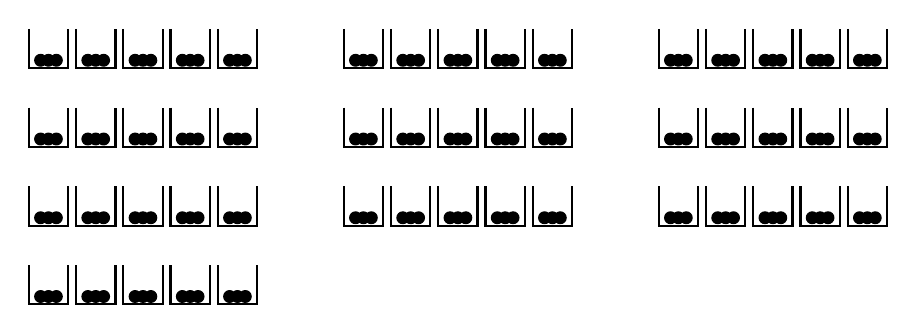
\begin{tikzpicture}[scale=0.5]
\newcommand\lax[3]{
\path[draw,thick,-] (#1-0.5,#2+0.5) -- (#1-0.5,#2-0.5) --
                    (#1+0.5,#2-0.5) -- (#1+0.5,#2+0.5);
\ifthenelse{\equal{#3}{1}}{\draw[fill=black] (#1,#2-0.3) circle (0.15);}{}
\ifthenelse{\equal{#3}{2}}{\draw[fill=black] (#1-0.2,#2-0.3) circle (0.15);}{}
\ifthenelse{\equal{#3}{2}}{\draw[fill=black] (#1+0.2,#2-0.3) circle (0.15);}{}
}
\newcommand\laa[7]{
    \lax{#1}{#2}{#3}
    \lax{#1+1.2}{#2}{#4}
    \lax{#1+2.4}{#2}{#5}
    \lax{#1+3.6}{#2}{#6}
    \lax{#1+4.8}{#2}{#7}
}

\laa{0}{0}{1}{1}{0}{0}{0}
\laa{0}{-2}{1}{0}{1}{0}{0}
\laa{0}{-4}{1}{0}{0}{1}{0}
\laa{0}{-6}{1}{0}{0}{0}{1}
\laa{8}{0}{0}{1}{1}{0}{0}
\laa{8}{-2}{0}{1}{0}{1}{0}
\laa{8}{-4}{0}{1}{0}{0}{1}
\laa{16}{0}{0}{0}{1}{1}{0}
\laa{16}{-2}{0}{0}{1}{0}{1}
\laa{16}{-4}{0}{0}{0}{1}{1}

\end{tikzpicture}
\end{center}

このシナリオでは答えは二項係数そのままです。${n \choose k}$となります。

シナリオ2:箱には複数の球を入れることができる。
例えば、$n = 5$ で $k = 2$の場合、解は15です。

\begin{center}
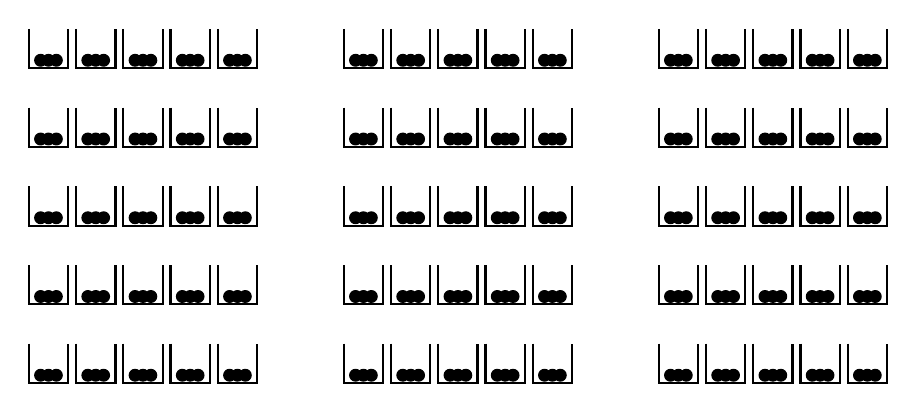
\begin{tikzpicture}[scale=0.5]
\newcommand\lax[3]{
\path[draw,thick,-] (#1-0.5,#2+0.5) -- (#1-0.5,#2-0.5) --
                    (#1+0.5,#2-0.5) -- (#1+0.5,#2+0.5);
\ifthenelse{\equal{#3}{1}}{\draw[fill=black] (#1,#2-0.3) circle (0.15);}{}
\ifthenelse{\equal{#3}{2}}{\draw[fill=black] (#1-0.2,#2-0.3) circle (0.15);}{}
\ifthenelse{\equal{#3}{2}}{\draw[fill=black] (#1+0.2,#2-0.3) circle (0.15);}{}
}
\newcommand\laa[7]{
    \lax{#1}{#2}{#3}
    \lax{#1+1.2}{#2}{#4}
    \lax{#1+2.4}{#2}{#5}
    \lax{#1+3.6}{#2}{#6}
    \lax{#1+4.8}{#2}{#7}
}

\laa{0}{0}{2}{0}{0}{0}{0}
\laa{0}{-2}{1}{1}{0}{0}{0}
\laa{0}{-4}{1}{0}{1}{0}{0}
\laa{0}{-6}{1}{0}{0}{1}{0}
\laa{0}{-8}{1}{0}{0}{0}{1}
\laa{8}{0}{0}{2}{0}{0}{0}
\laa{8}{-2}{0}{1}{1}{0}{0}
\laa{8}{-4}{0}{1}{0}{1}{0}
\laa{8}{-6}{0}{1}{0}{0}{1}
\laa{8}{-8}{0}{0}{2}{0}{0}
\laa{16}{0}{0}{0}{1}{1}{0}
\laa{16}{-2}{0}{0}{1}{0}{1}
\laa{16}{-4}{0}{0}{0}{2}{0}
\laa{16}{-6}{0}{0}{0}{1}{1}
\laa{16}{-8}{0}{0}{0}{0}{2}

\end{tikzpicture}
\end{center}

ボールを箱に入れる作業を
記号 ''o'' と ''$\rightarrow$''で表現しましょう。
はじめに、一番左の箱に立っているとする。記号 ''o'' は現在の箱に玉を入れることを意味し、
記号''$\rightarrow$''は次の右隣の箱に移動することを意味します。
この表記法を用いると、各解は''o''という記号を$k$回、
''$\rightarrow$''という記号を$n- 1$回含む文字列となります。
例えば、上の図の右上の解は、''$\rightarrow$ $\rightarrow$ o $\rightarrow$ o $\rightarrow$''
という文字列に相当します。
そのため答えば${k+n-1 \choose k}$です。

シナリオ3: 各箱にボールを入れる。しかし隣り合う箱にボールが入っていてはならない。
$n=5$, $k=2$とするとき、次の6通りが考えられます。

\begin{center}
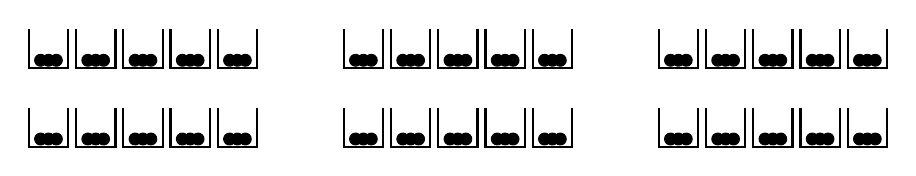
\begin{tikzpicture}[scale=0.5]
\newcommand\lax[3]{
\path[draw,thick,-] (#1-0.5,#2+0.5) -- (#1-0.5,#2-0.5) --
                    (#1+0.5,#2-0.5) -- (#1+0.5,#2+0.5);
\ifthenelse{\equal{#3}{1}}{\draw[fill=black] (#1,#2-0.3) circle (0.15);}{}
\ifthenelse{\equal{#3}{2}}{\draw[fill=black] (#1-0.2,#2-0.3) circle (0.15);}{}
\ifthenelse{\equal{#3}{2}}{\draw[fill=black] (#1+0.2,#2-0.3) circle (0.15);}{}
}
\newcommand\laa[7]{
    \lax{#1}{#2}{#3}
    \lax{#1+1.2}{#2}{#4}
    \lax{#1+2.4}{#2}{#5}
    \lax{#1+3.6}{#2}{#6}
    \lax{#1+4.8}{#2}{#7}
}

\laa{0}{0}{1}{0}{1}{0}{0}
\laa{0}{-2}{1}{0}{0}{1}{0}
\laa{8}{0}{1}{0}{0}{0}{1}
\laa{8}{-2}{0}{1}{0}{1}{0}
\laa{16}{0}{0}{1}{0}{0}{1}
\laa{16}{-2}{0}{0}{1}{0}{1}
\end{tikzpicture}
\end{center}

このシナリオでは、
$k$個のボールが箱に入れられ、
隣り合う2つの箱の間に空の箱があるとしましょう。
課題は、残りの空き箱の位置を選択することである。
このような箱は $n-2k+1$ 個あり、その位置は $k+1$ が考えられます。

ここでシナリオ2の式を思い出すと
${n-k+1 \choose n-2k+1}$であることがわかります。

\subsubsection{多項係数 - Multinomial coefficients}

\index{多項係数 - multinomial coefficient}

\key{多項係数 - multinomial coefficient}は、
\[ {n \choose k_1,k_2,\ldots,k_m} = \frac{n!}{k_1! k_2! \cdots k_m!}, \]
であり、$n$個の要素をサイズ $k_1,k_2,\ldots,k_m$の部分集合に分割できる方法の数に等しくなります。
この時、$k_1+k_2+\cdots+k_m=n$とします。

多項係数は二項係数の一般化と見ることができ、$m = 2$なら、上式は二項係数の式となります。

\section{カタラン数 - Catalan numbers}

\index{カタラン数 - Catalan number}

\key{カタラン数 - Catalan number}
$C_n$ は、$n$個の左括弧と$n$個の右括弧からなる有効な括弧式の数に等しいような数字です。
例えば$C_3=5$ですが、左右3つの括弧を使って次のような括弧式が作れます。

\begin{itemize}[noitemsep]
\item \texttt{()()()}
\item \texttt{(())()}
\item \texttt{()(())}
\item \texttt{((()))}
\item \texttt{(()())}
\end{itemize}

\subsubsection{括弧表現 - Parenthesis expressions}

\index{括弧表現 - parenthesis expression}

有効な括弧表現は次の定義で示されます。

\begin{itemize}
\item 空の括弧は有効です
\item 式$A$が有効であるとき、\texttt{(}$A$\texttt{)} は有効です
\item $A$と$B$が有効である時、$AB$は有効です
\end{itemize}

有効な括弧式のもう1つの特徴は、
このような式の任意の接頭辞を選ぶと、
そこに含まれる右括弧以上の左括弧が含まれていなければならないことです。
また、完全な式には、左括弧と右括弧が同じ数だけ含まれていなければなりません。

\subsubsection{公式1: Formula 1}

カタラン数は次の式で求めることができます。
\[ C_n = \sum_{i=0}^{n-1} C_{i} C_{n-i-1}.\]

この和は、式を2つの部分に分割して両方の部分が有効な式であり、
最初の部分ができるだけ短い空でないものの数を調べます。
任意の$i$について 、最初の部分は$i + 1$組の括弧を含むため式の数は次の値の積となる。

\begin{itemize}
\item $C_{i}$: 一番外側の括弧を除いた、最初の部分の括弧を使った式の組み立て方の数
\item $C_{n-i-1}$: 2番目の括弧を使った式の組み立て方の数
\end{itemize}

なお、$C_0=1$となります。
これは、ゼロ個の括弧の組を使って空の括弧式を構成することができるためです。

\subsubsection{Formula 2}

カタラン数は二項係数から求めることもできます。
\[ C_n = \frac{1}{n+1} {2n \choose n}\]

$n$個の左括弧と$n$個の右括弧を含む、有効とは限らない括弧式を構成する数は、
全部で${2n \choose n}$ です。
これかから有効でないものの数を計算します。

括弧式が有効でない場合というのは、
ある地点に置いて右括弧の数が左括弧の数を上回るような接頭辞でなければいけません。
ここで、そのような接頭辞に属するそれぞれの括弧を逆にしてみます。
例えば、\texttt{())()(} は接頭辞 \texttt{())}を含んでおり、
接頭辞を反転させる と \texttt{)((()(} となります。

これを行うと式は$n + 1$個の左括弧と$n - 1$個の右括弧で構成さます。
このような${2n \choose n+1}$の式は有効でない括弧式の数となります。
したがって、有効な括弧式の数は、次の式で計算できます。
\[{2n \choose n}-{2n \choose n+1} = {2n \choose n} - \frac{n}{n+1} {2n \choose n} = \frac{1}{n+1} {2n \choose n}.\]

\subsubsection{木の数え上げ - Counting trees}

Catalan numbers are also related to trees:
カタラン数は木とも関係があります。

\begin{itemize}
\item $n$個のノードを持つ二分木の数は$C_n$
\item $n$個のノードを持つ根付き木の数は$C_{n-1}$
\end{itemize}
\noindent
$C_3=5$です。さて二分木は次のようになります。

\begin{center}
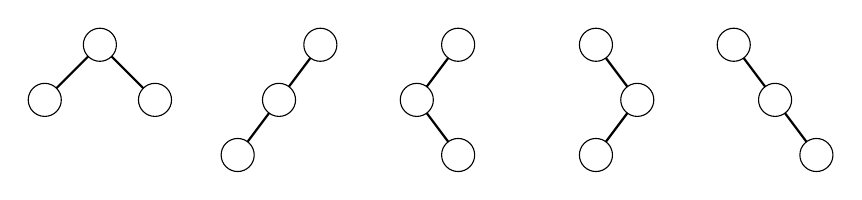
\begin{tikzpicture}[scale=0.7]
\path[draw,thick,-] (0,0) -- (-1,-1);
\path[draw,thick,-] (0,0) -- (1,-1);
\draw[fill=white] (0,0) circle (0.3);
\draw[fill=white] (-1,-1) circle (0.3);
\draw[fill=white] (1,-1) circle (0.3);

\path[draw,thick,-] (4,0) -- (4-0.75,-1) -- (4-1.5,-2);
\draw[fill=white] (4,0) circle (0.3);
\draw[fill=white] (4-0.75,-1) circle (0.3);
\draw[fill=white] (4-1.5,-2) circle (0.3);

\path[draw,thick,-] (6.5,0) -- (6.5-0.75,-1) -- (6.5-0,-2);
\draw[fill=white] (6.5,0) circle (0.3);
\draw[fill=white] (6.5-0.75,-1) circle (0.3);
\draw[fill=white] (6.5-0,-2) circle (0.3);

\path[draw,thick,-] (9,0) -- (9+0.75,-1) -- (9-0,-2);
\draw[fill=white] (9,0) circle (0.3);
\draw[fill=white] (9+0.75,-1) circle (0.3);
\draw[fill=white] (9-0,-2) circle (0.3);

\path[draw,thick,-] (11.5,0) -- (11.5+0.75,-1) -- (11.5+1.5,-2);
\draw[fill=white] (11.5,0) circle (0.3);
\draw[fill=white] (11.5+0.75,-1) circle (0.3);
\draw[fill=white] (11.5+1.5,-2) circle (0.3);
\end{tikzpicture}
\end{center}
根付き木は次のようになります。
\begin{center}
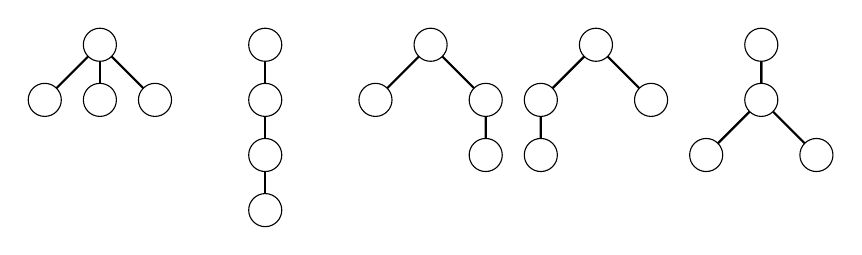
\begin{tikzpicture}[scale=0.7]
\path[draw,thick,-] (0,0) -- (-1,-1);
\path[draw,thick,-] (0,0) -- (0,-1);
\path[draw,thick,-] (0,0) -- (1,-1);
\draw[fill=white] (0,0) circle (0.3);
\draw[fill=white] (-1,-1) circle (0.3);
\draw[fill=white] (0,-1) circle (0.3);
\draw[fill=white] (1,-1) circle (0.3);

\path[draw,thick,-] (3,0) -- (3,-1) -- (3,-2) -- (3,-3);
\draw[fill=white] (3,0) circle (0.3);
\draw[fill=white] (3,-1) circle (0.3);
\draw[fill=white] (3,-2) circle (0.3);
\draw[fill=white] (3,-3) circle (0.3);

\path[draw,thick,-] (6+0,0) -- (6-1,-1);
\path[draw,thick,-] (6+0,0) -- (6+1,-1) -- (6+1,-2);
\draw[fill=white] (6+0,0) circle (0.3);
\draw[fill=white] (6-1,-1) circle (0.3);
\draw[fill=white] (6+1,-1) circle (0.3);
\draw[fill=white] (6+1,-2) circle (0.3);

\path[draw,thick,-] (9+0,0) -- (9+1,-1);
\path[draw,thick,-] (9+0,0) -- (9-1,-1) -- (9-1,-2);
\draw[fill=white] (9+0,0) circle (0.3);
\draw[fill=white] (9+1,-1) circle (0.3);
\draw[fill=white] (9-1,-1) circle (0.3);
\draw[fill=white] (9-1,-2) circle (0.3);

\path[draw,thick,-] (12+0,0) -- (12+0,-1) -- (12-1,-2);
\path[draw,thick,-] (12+0,0) -- (12+0,-1) -- (12+1,-2);
\draw[fill=white] (12+0,0) circle (0.3);
\draw[fill=white] (12+0,-1) circle (0.3);
\draw[fill=white] (12-1,-2) circle (0.3);
\draw[fill=white] (12+1,-2) circle (0.3);

\end{tikzpicture}
\end{center}

\section{包除原理 - Inclusion-exclusion}

\index{包除原理 - inclusion-exclusion}

\key{包除原理 - Inclusion-exclusion}
とは、集合の重なる部分の大きさが分かっているときに、
その集合の和の大きさを数えるテクニックです。
2つの集合の例としては、
\[ |A \cup B| = |A| + |B| - |A \cap B|,\]
となり、$A$と$B$は集合であり、$|X|$という表現は$X$の集合の大きさです。
これを図に示します。

\begin{center}
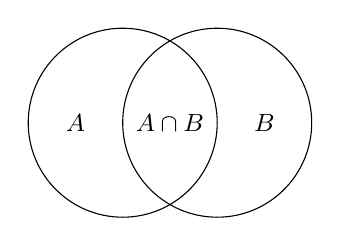
\begin{tikzpicture}[scale=0.8]

\draw (0,0) circle (1.5);
\draw (1.5,0) circle (1.5);

\node at (-0.75,0) {\small $A$};
\node at (2.25,0) {\small $B$};
\node at (0.75,0) {\small $A \cap B$};

\end{tikzpicture}
\end{center}

$A \cup B$の大きさを計算するには、少なくとも1つの円に属する領域の面積に対応する組合わせを計算することです。
図のようにまず$A$と$B$の面積から$A \cap B$の面積を差し引けば、
$A \cup B$の面積を計算することができます。

この考え方は集合の数が多くなっても同じ考え方ができます。
3つの集合の考え方と図を示します。
\[ |A \cup B \cup C| = |A| + |B| + |C| - |A \cap B|  - |A \cap C|  - |B \cap C| + |A \cap B \cap C| \]

\begin{center}
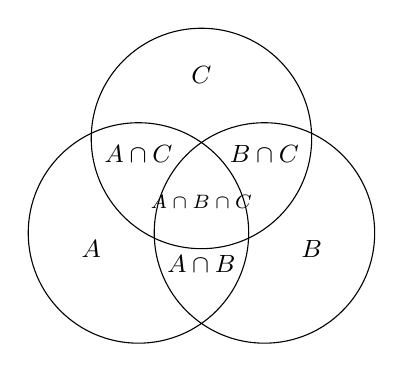
\begin{tikzpicture}[scale=0.8]

\draw (0,0) circle (1.75);
\draw (2,0) circle (1.75);
\draw (1,1.5) circle (1.75);

\node at (-0.75,-0.25) {\small $A$};
\node at (2.75,-0.25) {\small $B$};
\node at (1,2.5) {\small $C$};
\node at (1,-0.5) {\small $A \cap B$};
\node at (0,1.25) {\small $A \cap C$};
\node at (2,1.25) {\small $B \cap C$};
\node at (1,0.5) {\scriptsize $A \cap B \cap C$};

\end{tikzpicture}
\end{center}

一般的に$X_1 \cup X_2 \cup \cdots \cup X_n$のサイズの大きさは
集合$X_1,X_2,\ldots,X_n$の全ての重なる部分を調べることによって計算することができます。
この時に重なる部分の集合の数の偶奇に注目すると良いです。
交差点が奇数の集合を含む場合は加算、偶数の集合を含む場合は減算します。

また、重なる部分のサイズを計算する式は以下のようになります。
\[ |A \cap B| = |A| + |B| - |A \cup B|\]
集合が3つの場合は次のようになります。
\[ |A \cap B \cap C| = |A| + |B| + |C| - |A \cup B|  - |A \cup C|  - |B \cup C| + |A \cup B \cup C| .\]

\subsubsection{完全順列 - Derangements}

\index{完全順列 - derangement}

\key{完全順列 - derangements}とは、
$n$個の要素$\{1,2,\ldots,n\}$の並び替えのうち、
元の位置と一致する要素がないような順列のことです。
$n=3$とすると、2つの完全順列があり: $(2,3,1)$ と $(3,1,2)$です。

これを求める一つのアプローチとして、包除原理を用いることができます。
$X_k$ を位置 $k$ に要素 $k$ を含む並べ換えの集合としましょう。
例えば、$n = 3$ のとき、 集合は次のようになります。
\[
\begin{array}{lcl}
X_1 & = & \{(1,2,3),(1,3,2)\} \\
X_2 & = & \{(1,2,3),(3,2,1)\} \\
X_3 & = & \{(1,2,3),(2,1,3)\} \\
\end{array}
\]
これらを用いると、完全順列は以下に等しくなります。
\[ n! - |X_1 \cup X_2 \cup \cdots \cup X_n|, \]
この集合和の大きさを計算すれば十分になります。
包除原理を用いると、これは交点の大きさを計算すればよく、効率的に計算できます。
例えば、 $n=3$
$|X_1 \cup X_2 \cup X_3|$ のサイズは以下のようになります。
\[
\begin{array}{lcl}
 & & |X_1| + |X_2| + |X_3| - |X_1 \cap X_2|  - |X_1 \cap X_3|  - |X_2 \cap X_3| + |X_1 \cap X_2 \cap X_3| \\
 & = & 2+2+2-1-1-1+1 \\
 & = & 4, \\
\end{array}
\]
$3!-4=2$.とわかりました。

尚、この問題は包除原理を使わずに解けることがわかっています。
$f(n)$を$\{1,2,\ldots,n\}$に対応する完全順列の数とします。
この時、以下のように示せます。
\begin{equation*}
    f(n) = \begin{cases}
               0               & n = 1\\
               1               & n = 2\\
               (n-1)(f(n-2) + f(n-1)) & n>2 \\
           \end{cases}
\end{equation*}


この式は、完全順列の中で要素1がどのように変化するかのパターンを考えることで導き出すことができます。
要素1に代わる要素$x$の選び方は$n - 1$通りです。
それぞれの選択において、2つの選択肢がある。

\textit{Option 1:} 要素$x$を要素1に置き換える。この後、残る課題は、$n - 2$個
の要素からなる完全順列を構成することである。

\textit{Option 2:} 要素xを1以外の要素に置き換える。 
要素$x$を要素1に置き換えることはしないため、$n - 1$個の要素の完全順列を構成しなければならず、
他の要素もすべて変更しなければならなりません。

\section{バーンサイドの補題 - Burnside's lemma}

\index{バーンサイドの補題 - Burnside's lemma}

\key{バーンサイドの補題 - Burnside's lemma}
%\footnote{Actually, Burnside did not discover this lemma; he only mentioned it in his book \cite{bur97}.}
は、
対称的な組み合わせのグループごとに重複がないように組み合わせの数を数えるために利用します。
バーンサイドの補題は組み合わせの数が、
\[\sum_{k=1}^n \frac{c(k)}{n},\]
で示され、組み合わせの位置を変える方法が$n$通りあり、
そこに$k$ 番目の方法を適用しても変化しない$c(k)$ の組み合わせがあるとします。

例えば、真珠の色が$m$色あるとして、$n$個の真珠を使ったネックレスの組み合わせ数を計算してみましょう。
2つのネックレスが回転して似ている場合、対称(ここでは同一)であると言えます。

\begin{center}
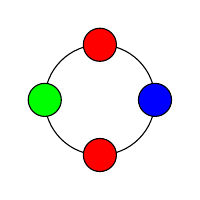
\begin{tikzpicture}[scale=0.7]
\draw[fill=white] (0,0) circle (1);
\draw[fill=red] (0,1) circle (0.3);
\draw[fill=blue] (1,0) circle (0.3);
\draw[fill=red] (0,-1) circle (0.3);
\draw[fill=green] (-1,0) circle (0.3);
\end{tikzpicture}
\end{center}
に対して、以下のネックレスは同一であるとしましょう。
\begin{center}
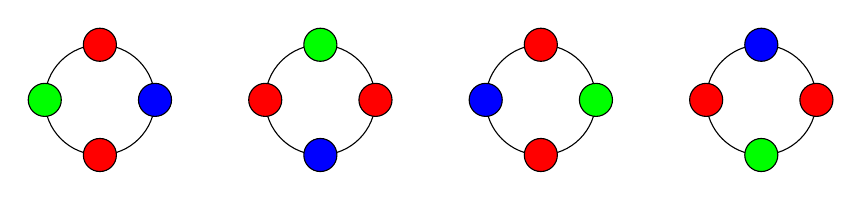
\begin{tikzpicture}[scale=0.7]
\draw[fill=white] (0,0) circle (1);
\draw[fill=red] (0,1) circle (0.3);
\draw[fill=blue] (1,0) circle (0.3);
\draw[fill=red] (0,-1) circle (0.3);
\draw[fill=green] (-1,0) circle (0.3);

\draw[fill=white] (4,0) circle (1);
\draw[fill=green] (4+0,1) circle (0.3);
\draw[fill=red] (4+1,0) circle (0.3);
\draw[fill=blue] (4+0,-1) circle (0.3);
\draw[fill=red] (4+-1,0) circle (0.3);

\draw[fill=white] (8,0) circle (1);
\draw[fill=red] (8+0,1) circle (0.3);
\draw[fill=green] (8+1,0) circle (0.3);
\draw[fill=red] (8+0,-1) circle (0.3);
\draw[fill=blue] (8+-1,0) circle (0.3);

\draw[fill=white] (12,0) circle (1);
\draw[fill=blue] (12+0,1) circle (0.3);
\draw[fill=red] (12+1,0) circle (0.3);
\draw[fill=green] (12+0,-1) circle (0.3);
\draw[fill=red] (12+-1,0) circle (0.3);
\end{tikzpicture}
\end{center}
まず、ネックレスを時計回りに$0,1,\ldots,n-1$ ステップ回転させることができるので、 
ネックレスの位置を変える方法は$n$通りあります。
ステップ数が0の場合、$m^n$ のネックレスはすべて同じで、
ステップ数が1の場合、各真珠の色が同じである$m$個のネックレスだけが同じままである。

より一般的には、ステップ数を$k$としたとき、合計で
\[m^{\textrm{gcd}(k,n)}\]
のネックレスが同じになります。
$\textrm{gcd}(k,n)$は$k$と$n$の最大公約数です。
この理由は、$\textrm{gcd}(k,n)$の大きさの真珠のブロックは互いに置き換えられるためです。
したがって、バーンサイドの補題によれば、首飾りの個数は
\[\sum_{i=0}^{n-1} \frac{m^{\textrm{gcd}(i,n)}}{n}. \]
で示され、長さ4, 色が3なら、以下の通りとなります。
\[\frac{3^4+3+3^2+3}{4} = 24. \]

\section{ケイリーの公式 - Cayley's formula}

\index{ケイリーの公式 - Cayley's formula}

\key{ケイリーの公式 - Cayley's formula}
% \footnote{While the formula is named after A. Cayley,
% who studied it in 1889, it was discovered earlier by C. W. Borchardt in 1860.}
は、$n$個のノードを含む$n^{n-2}$のラベル付き木が存在することを述べている。
ノードは$1,2,\ldots,n$とラベル付けされ、
2つの木はその構造かラベルが異なれば異なる木としましょう。

\begin{samepage}
例えば、$n = 4$のとき、ラベル付き木の本数は$4^{4-2}=16$となる。
\begin{center}
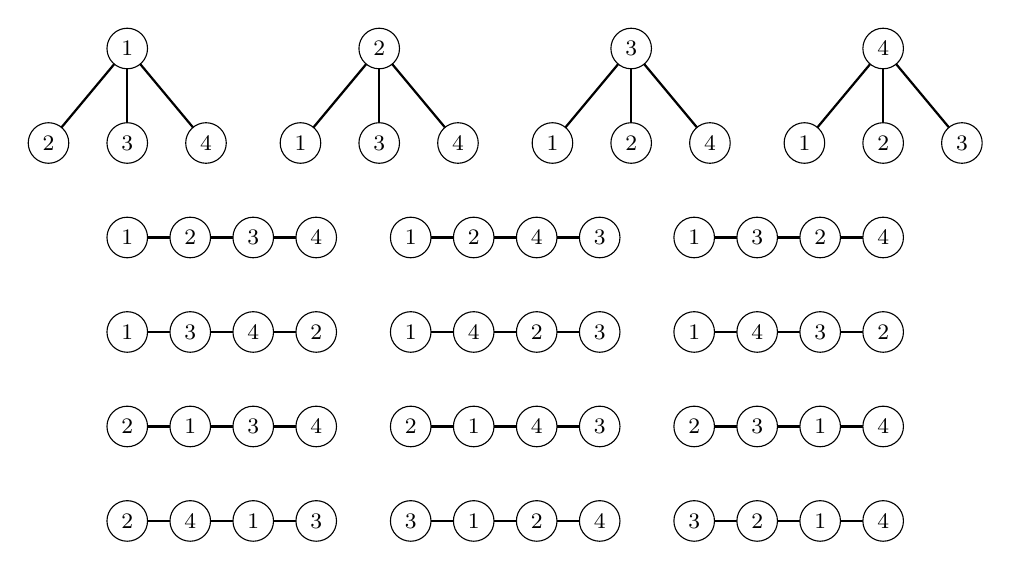
\begin{tikzpicture}[scale=0.8]
\footnotesize

\newcommand\puua[6]{
\path[draw,thick,-] (#1,#2) -- (#1-1.25,#2-1.5);
\path[draw,thick,-] (#1,#2) -- (#1,#2-1.5);
\path[draw,thick,-] (#1,#2) -- (#1+1.25,#2-1.5);
\node[draw, circle, fill=white] at (#1,#2) {#3};
\node[draw, circle, fill=white] at (#1-1.25,#2-1.5) {#4};
\node[draw, circle, fill=white] at (#1,#2-1.5) {#5};
\node[draw, circle, fill=white] at (#1+1.25,#2-1.5) {#6};
}
\newcommand\puub[6]{
\path[draw,thick,-] (#1,#2) -- (#1+1,#2);
\path[draw,thick,-] (#1+1,#2) -- (#1+2,#2);
\path[draw,thick,-] (#1+2,#2) -- (#1+3,#2);
\node[draw, circle, fill=white] at (#1,#2) {#3};
\node[draw, circle, fill=white] at (#1+1,#2) {#4};
\node[draw, circle, fill=white] at (#1+2,#2) {#5};
\node[draw, circle, fill=white] at (#1+3,#2) {#6};
}

\puua{0}{0}{1}{2}{3}{4}
\puua{4}{0}{2}{1}{3}{4}
\puua{8}{0}{3}{1}{2}{4}
\puua{12}{0}{4}{1}{2}{3}

\puub{0}{-3}{1}{2}{3}{4}
\puub{4.5}{-3}{1}{2}{4}{3}
\puub{9}{-3}{1}{3}{2}{4}
\puub{0}{-4.5}{1}{3}{4}{2}
\puub{4.5}{-4.5}{1}{4}{2}{3}
\puub{9}{-4.5}{1}{4}{3}{2}
\puub{0}{-6}{2}{1}{3}{4}
\puub{4.5}{-6}{2}{1}{4}{3}
\puub{9}{-6}{2}{3}{1}{4}
\puub{0}{-7.5}{2}{4}{1}{3}
\puub{4.5}{-7.5}{3}{1}{2}{4}
\puub{9}{-7.5}{3}{2}{1}{4}
\end{tikzpicture}
\end{center}
\end{samepage}

次に、プリュファーコードを使ってケイリーの公式がどのように導かれるのかを見ていきます。

\subsubsection{プリューファー列 - Prüfer code}

\index{プリューファー列 - Prüfer code}

A \key{プリューファー列 - Prüfer code}
%\footnote{In 1918, H. Prüfer proved Cayley's theorem using Prüfer codes \cite{pru18}.}
ラベル付きツリーを記述する$n - 2$個の数列です。
この数列は木から$n - 2$枚の葉を除去する過程を経て構成されます。
各ステップで、最も小さいラベルを持つ葉が取り除かれ、
その唯一の隣接葉のラベルをコードに追加します。

例えば、次のようなグラフのプルーファーコードを計算してみましょう。
\begin{center}
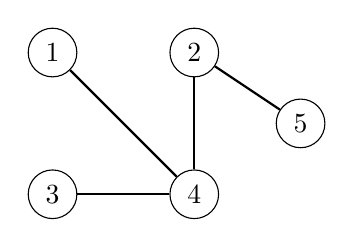
\begin{tikzpicture}[scale=0.9]
\node[draw, circle] (1) at (2,3) {$1$};
\node[draw, circle] (2) at (4,3) {$2$};
\node[draw, circle] (3) at (2,1) {$3$};
\node[draw, circle] (4) at (4,1) {$4$};
\node[draw, circle] (5) at (5.5,2) {$5$};

\path[draw,thick,-] (1) -- (4);
\path[draw,thick,-] (3) -- (4);
\path[draw,thick,-] (2) -- (4);
\path[draw,thick,-] (2) -- (5);
\end{tikzpicture}
\end{center}

まず、ノード1を削除し、ノード4をコードに追加します。
\begin{center}
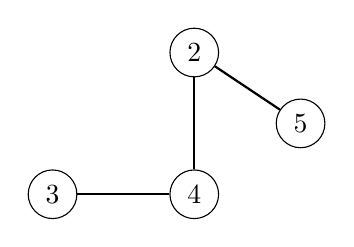
\begin{tikzpicture}[scale=0.9]
%\node[draw, circle] (1) at (2,3) {$1$};
\node[draw, circle] (2) at (4,3) {$2$};
\node[draw, circle] (3) at (2,1) {$3$};
\node[draw, circle] (4) at (4,1) {$4$};
\node[draw, circle] (5) at (5.5,2) {$5$};

%\path[draw,thick,-] (1) -- (4);
\path[draw,thick,-] (3) -- (4);
\path[draw,thick,-] (2) -- (4);
\path[draw,thick,-] (2) -- (5);
\end{tikzpicture}
\end{center}

そして、ノード3を削除し、ノード4を追加するコードになります。
\begin{center}
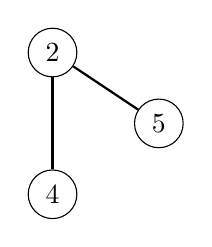
\begin{tikzpicture}[scale=0.9]
%\node[draw, circle] (1) at (2,3) {$1$};
\node[draw, circle] (2) at (4,3) {$2$};
%\node[draw, circle] (3) at (2,1) {$3$};
\node[draw, circle] (4) at (4,1) {$4$};
\node[draw, circle] (5) at (5.5,2) {$5$};

%\path[draw,thick,-] (1) -- (4);
%\path[draw,thick,-] (3) -- (4);
\path[draw,thick,-] (2) -- (4);
\path[draw,thick,-] (2) -- (5);
\end{tikzpicture}
\end{center}

最後にノード4を削除し、ノード2をコードに追加します。
\begin{center}
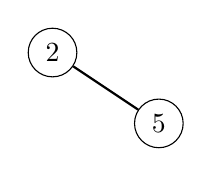
\begin{tikzpicture}[scale=0.9]
%\node[draw, circle] (1) at (2,3) {$1$};
\node[draw, circle] (2) at (4,3) {$2$};
%\node[draw, circle] (3) at (2,1) {$3$};
%\node[draw, circle] (4) at (4,1) {$4$};
\node[draw, circle] (5) at (5.5,2) {$5$};

%\path[draw,thick,-] (1) -- (4);
%\path[draw,thick,-] (3) -- (4);
%\path[draw,thick,-] (2) -- (4);
\path[draw,thick,-] (2) -- (5);
\end{tikzpicture}
\end{center}

このグラフのプリューファー列は$[4,4,2]$です。

どのような木に対してもプリューファー列を構成することができます。
さらに重要なことは、プリューファー列から元の木を再構成することができることです。
したがって、ノード数$n$のラベル付き木の数は、
サイズ$n$ のプリュファー列の数 $n^{n-2}$に等しくなります。
